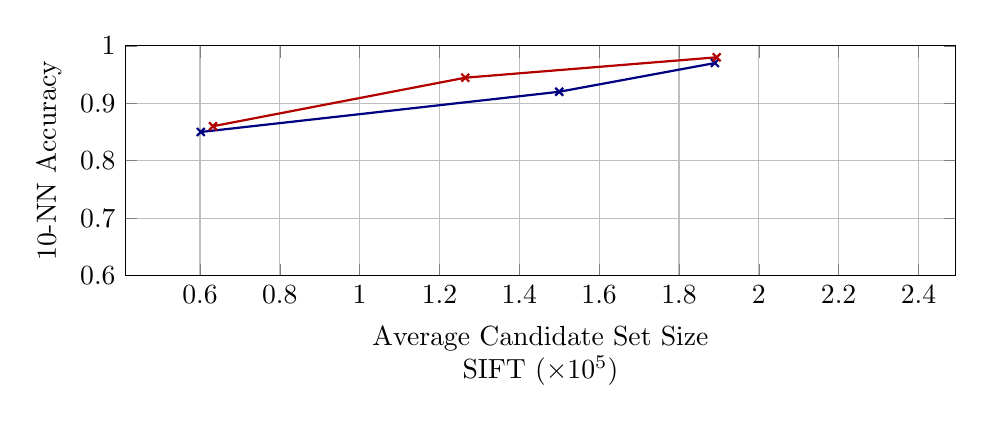
\begin{tikzpicture}
        \begin{axis}[
            width=\linewidth,
            height=4.5cm,
            grid=major,
			xlabel={\begin{tabular}{@{}c@{}}Average Candidate Set Size\\ SIFT ($\times 10^5$)\end{tabular}},
            ylabel={10-NN Accuracy},
            mark options={solid},
            xtick scale label code/.code={},
            xticklabel style={align=center},
            ymin=0.6,
            ymax=1,
            xmax=249300
        ]
        
        % Original
        \addplot[blue!50!black, thick, mark=x, mark size=2pt] coordinates {
            (60200, 0.85)
            (150000, 0.92)
            (189000, 0.97)
        };
        % PCA
        \addplot[red!70!black, thick, mark=x, mark size=2pt] coordinates {
            (63243, 0.86)
            (126475, 0.9445)
            (189444, 0.98)
        };
        \end{axis}
\end{tikzpicture}